\documentclass[12pt,a4paper]{article}
\usepackage[T2A]{fontenc}
\usepackage[utf8]{inputenc}
\usepackage[russian]{babel}

\usepackage{graphicx}
\graphicspath{{imgs/}}
\DeclareGraphicsExtensions{.png}

\usepackage{float}
\usepackage{hyperref}

\usepackage{listings}
\lstset{
      language=Matlab,
      inputpath=m,
      extendedchars=true,
      keepspaces=true,
      breaklines=true,
      basicstyle=\small\ttfamily,
      literate={а}{{\selectfont\char224}}1
               {б}{{\selectfont\char225}}1
               {в}{{\selectfont\char226}}1
               {г}{{\selectfont\char227}}1
               {д}{{\selectfont\char228}}1
               {е}{{\selectfont\char229}}1
               {ё}{{\"e}}1
               {ж}{{\selectfont\char230}}1
               {з}{{\selectfont\char231}}1
               {и}{{\selectfont\char232}}1
               {й}{{\selectfont\char233}}1
               {к}{{\selectfont\char234}}1
               {л}{{\selectfont\char235}}1
               {м}{{\selectfont\char236}}1
               {н}{{\selectfont\char237}}1
               {о}{{\selectfont\char238}}1
               {п}{{\selectfont\char239}}1
               {р}{{\selectfont\char240}}1
               {с}{{\selectfont\char241}}1
               {т}{{\selectfont\char242}}1
               {у}{{\selectfont\char243}}1
               {ф}{{\selectfont\char244}}1
               {х}{{\selectfont\char245}}1
               {ц}{{\selectfont\char246}}1
               {ч}{{\selectfont\char247}}1
               {ш}{{\selectfont\char248}}1
               {щ}{{\selectfont\char249}}1
               {ъ}{{\selectfont\char250}}1
               {ы}{{\selectfont\char251}}1
               {ь}{{\selectfont\char252}}1
               {э}{{\selectfont\char253}}1
               {ю}{{\selectfont\char254}}1
               {я}{{\selectfont\char255}}1
               {А}{{\selectfont\char192}}1
               {Б}{{\selectfont\char193}}1
               {В}{{\selectfont\char194}}1
               {Г}{{\selectfont\char195}}1
               {Д}{{\selectfont\char196}}1
               {Е}{{\selectfont\char197}}1
               {Ё}{{\"E}}1
               {Ж}{{\selectfont\char198}}1
               {З}{{\selectfont\char199}}1
               {И}{{\selectfont\char200}}1
               {Й}{{\selectfont\char201}}1
               {К}{{\selectfont\char202}}1
               {Л}{{\selectfont\char203}}1
               {М}{{\selectfont\char204}}1
               {Н}{{\selectfont\char205}}1
               {О}{{\selectfont\char206}}1
               {П}{{\selectfont\char207}}1
               {Р}{{\selectfont\char208}}1
               {С}{{\selectfont\char209}}1
               {Т}{{\selectfont\char210}}1
               {У}{{\selectfont\char211}}1
               {Ф}{{\selectfont\char212}}1
               {Х}{{\selectfont\char213}}1
               {Ц}{{\selectfont\char214}}1
               {Ч}{{\selectfont\char215}}1
               {Ш}{{\selectfont\char216}}1
               {Щ}{{\selectfont\char217}}1
               {Ъ}{{\selectfont\char218}}1
               {Ы}{{\selectfont\char219}}1
               {Ь}{{\selectfont\char220}}1
               {Э}{{\selectfont\char221}}1
               {Ю}{{\selectfont\char222}}1
               {Я}{{\selectfont\char223}}1
               }

\usepackage{amsmath}
\usepackage{amsfonts}
\usepackage{amssymb}
\documentclass[10pt,a4paper]{report}
\usepackage[utf8x]{inputenc}
\usepackage[russian]{babel}
\usepackage[OT1]{fontenc}
\usepackage{amsmath}
\usepackage{subfig}
\usepackage{amsfonts}
\usepackage{amssymb}
\usepackage{graphicx}
\usepackage{placeins}
\usepackage{enumerate}
\usepackage{float}

\usepackage[shortlabels]{enumitem}


\usepackage{listings}
\usepackage[framed,numbered,autolinebreaks,useliterate]{mcode}
\usepackage[left=2cm,right=2cm,top=2cm,bottom=2cm]{geometry}

\renewcommand{\thesubsection}{\arabic{subsection}}
\makeatletter
\def\@seccntformat#1{\@ifundefined{#1@cntformat}%
	{\csname the#1\endcsname\quad}%       default
	{\csname #1@cntformat\endcsname}}%    enable individual control
\newcommand\section@cntformat{}
\makeatother
\renewcommand\lstlistingname{Listing}
\begin{document}
	\begin{titlepage}
		\begin{center}
			% Шапка
			Санкт-Петербургский государственный политехнический \\ университет Петра Великого \\[0.1cm]
			Кафедра компьютерных систем и программных технологий \\[9cm]
			
			% Основная часть
			\textbf{Отчет по Лабораторной работе 7}\\[0.1cm]
			\textbf{Дисциплина:} Телекоммуникационные технологии \\[0.1cm]
			\textbf{Тема:} Помехоустойчивое кодирование
		\end{center}
		
		\vfill
		
		% Имена/подписи
		\flushleft{Выполнил студент гр. 33501/1} \hfill\parbox{8cm}{
			\hspace*{3cm}\hbox to 0cm{\raisebox{-1em}{\small(подпись)}}\hspace*{-0.8cm}\rule{3cm}{0.8pt} Поляков К.О.}\\[0.6cm]
		
		\flushleft{Преподаватель} \hfill\parbox{8cm}{
			\hspace*{3cm}\hbox to 0cm{\raisebox{-1em}{\small(подпись)}}\hspace*{-0.8cm}\rule{3cm}{0.8pt} Богач Н.В.}\\[0.6cm]
		
		\hfill\parbox{9cm}{\hspace*{3cm}``\rule{0.7cm}{0.8pt}''\rule{3cm}{0.8pt}~2017 г.}
		
		\vfill
		
		\begin{center}
			% Bottom of the page
			Санкт-Петербург \par
			2017 г.
		\end{center}
	\end{titlepage}
\newpage

\section{Помехоустойчивое кодирование}

\subsection{Цель работы}

  Изучение методов помехоустойчивого кодирования, а также сравнение их свойств.

\subsection{Постановка задачи}

	\begin{enumerate}
	  \item Провести кодирование/декодирование сигнала, полученного с помощью функции randerr кодом Хэмминга двумя способами: с помощью встроенных функций encode/decode, а также через создание проверочной и генераторной матриц и вычисление синдрома. Оценить корректирующую способность кода.
    \item Выполнить кодирование/декодирование циклическим кодом, БЧХ-кодом, кодом Рида-Соломона. Оценить корректирующую способность кода.
	\end{enumerate}
	
\subsection{Справочные материалы}
  \begin{itemize}
    \item Солопченко Г.Н. Теория информации. СПб.: Изд-во Политехнического унив., 2010. С. 36-55;
    \item Темников Ф. Е., Афонин В. А., Дмитриев В. И. Теоретические основы информационной техники. М.: Энергия, 1971. С. 96-177;
    \item Кузьмин И.В., Кедрус В.А. Основы теории информации и кодирования. К.: Вища шк. Головное изд-во, 1986. С. 79-104.
  \end{itemize}

\subsection{Теоретические положения}
  
  Битовые ошибки в каналах связи нельзя исключить полностью, даже если выбранный способ кодирования дискретного сигнала код обеспечивает хорошую степень синхронизации и высокий уровень отношения сигнала к шуму. Поэтому при передаче дискретной информации применяются специальные коды, которые позволяют обнаруживать (а иногда даже исправлять) битовые ошибки.
  
  Преимуществом цифровых методов записи, воспроизведения и передачи аналоговой информации является возможность контроля достоверности считанных с носителя или полученных по линии связи данных. Для этого можно применять те же методы, что и в случае компьютерных данных,~-- вычисление контрольной суммы, повторная передача искаженных кадров, применение самокорректирующихся кодов.
  
  Распознавание и коррекцию искаженных данных сложно осущест\-вить средствами физического уровня, поэтому чаще всего эту работу берут на себя протоколы, лежащие выше: канальный, сетевой, транспортный или прикладной. В то же время распознавание ошибок на физическом уровне экономит время, так как приемник не ждет полного помещения кадра в буфер, а отбраковывает его сразу при распознавании ошибочных битов внутри кадра.
  
  Есть два подхода работы протоколов. Протоколы, реализующие первый принцип, обеспечивают надежность за счет повторной передачи искаженных или потерянных пакетов. Такие протоколы основаны на том, что приемник в состоянии распознать факт искажения информации в принятом кадре. Еще одним, более эффективным подходом, чем повторная передача пакетов, является использование самокорректирующихся кодов, которые позволяют не только обнаруживать, но и исправлять ошибки в принятом кадре.
  
\subsubsection{Классификация помехоустойчивого кодирования}
  
  Помехоустойчивость кодирования обеспечивается за счет введения \emph{избыточности} в кодовые комбинации. Избыточность позволяет наложить на передаваемые последовательности символов дополнительные условия, проверка которых на приемной стороне дает возможность обнаружить и исправить ошибки, возникающих в результате влияния помех.
  
  Все помехоустойчивые коды можно разделить на два основных класса: \emph{блочные} и \textit{непрерывные} (Рис.~\ref{img:t:class}).

  В блочных кодах каждому сообщения (или его элементу) сопоставляется кодовая комбинация (блок) из определенного количества сигналов. Блоки кодируются и декодируются отдельно друг от друга.
  
  \begin{figure}[!ht]
	  \centering
	  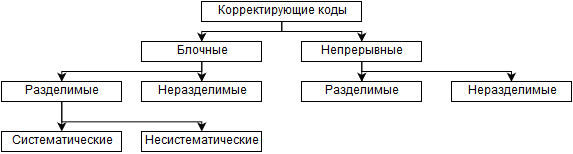
\includegraphics[width=\linewidth]{class}
	  \caption{Классификация помехоустойчивых кодов.}
	  \label{img:t:class}
  \end{figure}
  
  Блочные коды могут быть равномерными, когда длина $n$ кодовых комбинаций постоянна, или неравномерными, когда $n$ постоянно. Неравномерные помехоустойчивые коды не получили практического применения из-за сложности их технической реализации.
  
  В непрерывных кода введение избыточности в последовательность входных символов осуществляется без разбивки ее на отдельные блоки. Процессы кодирования и декодирования в непрерывных кодах имеют также непрерывный характер.
  
  Как блочные, так и непрерывные коды в зависимости от методов внесения избыточности подразделяются на \emph{разделимые} и \emph{неразделимые}. В разделимых кодах четко разграничена роль отдельных символов. Одни символы являются информационными, другие~-- проверочными и служат для обнаружения и исправления ошибок.
  
  В неразделимых кодах раз­деление информационной и проверочной части невозможно, что затрудняет декодирование, особенно при необходимости исправления ошибок. К таким кодам относятся коды с постоянным весом и некото­рые другие.
  
  Разделимые коды делятся на \emph{систематические} и \emph{несистематические}. Систематические коды характеризуются тем, что сумма по модулю 2 двух разрешенных комбинаций дает комбинацию того же кода. Процессы кодирования и декодирования в систематических кодах  сводятся к подсчету сумм по модулю 2 информационных и проверочных символов в различных сочетаниях.

  Несистематические коды, к числу которых относятся коды с суммированием, указанным выше свойством не обладают. Метод построения таких кодов состоит в том, что проверочные символы определяются как результат суммирования символов, входящих в кодовую комбинацию или ее часть.

  Разновидностью систематических кодов являются циклические коды, характеризующиеся тем, что циклическая перестановка всех символов одной комбинации дает другую комбинацию, принадлежащую этому же коду.

  Принципиально все перечисленные коды могут быть использованы как для обнаружения, так и для  исправления ошибок. Однако отмеченные выше удобства построения кодирующих и декодирующих устройств  определили преимущественное  применение  лишь  некоторых из них.
  
\subsubsection{Связь корректирующей способности кода с кодовым расстоянием}
  
  Блоковые (равномерные) коды характеризуются так называемым \emph{минимальным кодовым расстоянием}. Количеством единиц в кодовой комбинации называют \emph{весом кодовой комбинации} и обозначают $w$. Например, кодовая комбинация $100101100$ характеризуется длиной $n=9$ и весом $w=4$.
  
  Степень отличия любых двух кодовых комбинация данного кода характеризуется так называемым \emph{расстоянием между кодами} $d$. Для двоичного кода под данным термином понимается \emph{расстояние Хэмминга}. Оно выражается числом позиций или символов, в которых  комбинации отличаются одна от другой, и определяется как вес суммы по модулю два этих кодовых комбинация. Например, для определения расстояния между комбинациями $100101100$ и $110110101$ необходимо просуммировать их по модулю два: $1\dot{0}01\dot{0}\dot{1}10\dot{0}\oplus 1\dot{1}01\dot{1}\dot{0}10\dot{1}=010011001$ (точками выделены отличающиеся биты).
  
  Полученная в результате суммирования новая кодовая комбинация характеризуется весом $w=4$. Следовательно, расстояние Хэмминга $d=4$. При этом в качестве \emph{минимального кодового расстояния} $d_\text{мин}$ выбирается наименьшее из всех расстояний по Хэммингу для любых пар различных кодовых слов, образующих код. $d_\text{мин}$~-- очень важная характеристика кода, ибо именно она характеризует его \emph{корректирующую способность}:
  \begin{equation}
    \nonumber
    t=\left\lfloor\frac{d_\text{мин}-1}{2}\right\rfloor\text{, здесь угловые скобки обозначают округление вниз.}
  \end{equation}
  
  Код, образованный различными $N=2^n$ кодовыми словами длиной n, имеет $d=1$. Этот код не обладает свойством избыточности и не предоставляет возможности обнаруживать или исправлять ошибки, потому что ошибка при передаче одного символа переводит одно слово этого кода в другое кодовое слово. Это наглядно показано на Рис.~\ref{img:t:d},~а), где жирными точками отмечены кодовые слова, отстоящие друг от друга на расстоянии, равном 1. Кодовые  слова,  расстояние  между  которыми  равно 2, показаны  жирными точками на Рис.~\ref{img:t:d},~б). Это разрешенные кодовые слова. Остальные точки изображают неразрешенные кодовые слова, отсутствующие в коде.
  \begin{figure}[H]
	  \centering
	  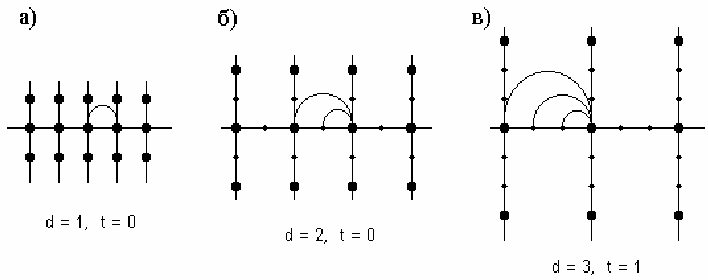
\includegraphics[width=\linewidth]{d}
	  \caption{Кодовое расстояние и ошибки в передаче кодовых слов.}
	  \label{img:t:d}
  \end{figure}
  
  Из Рис.~\ref{img:t:d},~б) видно, что код с расстоянием 2 дает возможность обнаружить  одну  ошибку,  поскольку  одна  ошибка  приводит  любое  разрешенное кодовое слово к неразрешенному. Ошибки в двух позициях переводят кодовое слово в другое слово из этого же кода, и эти  ошибки обнаружены  быть  не  могут.  На  Рис.~\ref{img:t:d},~в) изображены  разрешенные  кодовые слова с расстоянием между ними, равном 3. Из рисунка видно, что такой код  допускает  исправление  одной  ошибки  и  обнаружение  двух  ошибок.
   
   В общем случае при необходимости \emph{обнаружить} ошибки кратности $r$ (т.е. количества искаженных символов в в кодовой комбинации) минимальное хэмингово расстояние между разрешенными кодовыми комбинациями должно быть по крайней мере на единцу больше $r$, т.е $d_{\text{мин}}\geq r+1$.
   
   Для \emph{исправления} ошибок кратности $s$ минимальное хэмингово расстояние между разрешенными комбинациями должно удовлетворять соотношению $d_{\text{мин}}\geq 2s+1$. Т.е. для исправления одиночно ошибки каждой разрешенной кодовой комбинации необходимо сопоставить свое подмножество запрещенных кодовых комбинаций, состоящее из $d_{\text{мин}}=3$ кодов. Для $n=3$ за разрешенные комбинации можно, например, принять $000$ и $111$. Тогда для $000$ запрещенными будут $001$, $010$ и $100$, а для $111$~-- $110$, $101$ и $011$.
   
   В реальных каналах связи длительность импульсов помехи может превышать длительность символа. При этом одновременно искажаются несколько расположенных рядом символов комбинации. Ошибки такого рода получили название пачек ошибок или пакетов ошибок. Длиной пачки ошибок называется число следующих друг за другом символов, левее и правее которых в кодовой комбинации искаженных символов не содержится.
   
\subsubsection{Показатели качества корректирующего кода}
  
  Любой корректирующий код характеризуется рядом показателей: 
  \begin{itemize}
    \item длиной $n$;
    \item основанием $m$;
    \item количеством информационных символов $i$;
    \item количеством корректирующих символов $k$;
    \item полным числом всех возможных кодовых комбинаций $N=m^n$;
    \item числом разрешенных кодовых комбинаций (мощностью кода) $N_\text{р}$;
    \item весом кодовой комбинации $w$;
    \item кодовым расстоянием $d$;
    \item наименьшим расстоянием между разрешенными кодовыми комбинациями $d_\text{мин}$;
    \item и пр.
  \end{itemize}
  
  Однако одной из основных характеристик корректирующего кода является избыточность кода. Для того, чтобы код приобрел способность к обнаружению и коррекции ошибок, необходимо отказаться от его безызбыточности. Для этого и разделяют всё множество возможных комбинаций двоичных символов на два подмножества, как уже говорилось ранее: \emph{допустимых} кодовых слов и \emph{недопустимых}. Разбиение осуществляется таким образом, чтобы увеличить минимальное кодовое расстояние между допустимыми словами. В этом случае любая однократная ошибка превращает допустимое кодовое слово в недопустимое, что позволяет ее обнаружить.
  
  Естественно, что введение дополнительных контрольных разрядов увеличивает затраты на хранение или передачу кодированной информации. При этом фактический объем полезной информации остается неизменным. В этом случае можно говорить об избыточности помехоустойчивого кода, которую формально можно определить как отношение числа контрольных разрядов к общему числу разрядов кодового слова:
  \begin{equation}
    \nonumber
    R_n=k/n*100\%\text{,}
  \end{equation}
где $k$~-- число контрольных разрядов, а $n$~-- общее число бит комбинации.
  
  Пожалуй, основным показателем качества корректирующего кода является его способность обеспечить правильный прием кодовых комбинаций при наличии искажений под воздействием помех, т.е. \emph{помехоустойчивость кода}.
  
  Количественная оценка помехоустойчивости кода может быть осуществлена по-разному. Можно использовать вероятность правильного приема кодовых комбинаций $P_\text{пр}=1-P_\text{ош}$, где $P_\text{ош}$~-- вероятность ошибочного приема кодовых комбинаций.
  
  Если код не обладает корректирующими свойствами, то вероятность ошибочного према $P_\text{ош}$ будет равна вероятности искажения кодовых комбинаций $P_k$. Для корректирующего кода $P_\text{ош}<P_k$. В реальных условиях $P_\text{ош}\leq 1$, поэтому более удобным критерием оценки помехоустойчивости кода является логарифмическая величина
  \begin{equation}
    \nonumber
    S_k=\lg{\frac{1}{P_\text{ош}}}=\lg{\frac{1}{1-P_\text{пр}}}\text{.}
  \end{equation}
  
\subsubsection{Коды Хэмминга}
  
  Коды Хемминга эффективно обнаруживают и исправляют изолированные ошибки, то есть отдельные искаженные биты, которые разделены большим количеством корректных битов. Однако при появлении длинной последовательности искаженных битов (пульсации ошибок) коды Хемминга не работают.
  
  Для каждого числа проверочных символов используется специальная маркировка вида $(n, i)$, где $n$~-- количество символов в сообщении, $i$~-- количество информационных символов в сообщении. Например, существуют коды $(7, 4)$, $(15, 11)$, $(31, 26)$. Каждый проверочный символ в коде Хэмминга представляет сумму по модулю $2$ некоторой подпоследовательности данных. Например, когда количество информационных бит $i$ в блоке равно $4$~-- это код $(7,4)$, количество проверочных символов $k=3$. Классически, эти символы располагаются на позициях, равных степеням двойки в порядке возрастания и формируют коды $(2^k-1,2^k-1-k)$.
  
  В итоге, код Хэмминга должен иметь минимальное кодовое расстояние $d_\text{мин}=3$. Длина кода $n$ выбирается из условия $2^i\leq 2^n/(1+n)$, где $i$~-- количество информационных сигналов.
  
  Код строится таким образом, чтобы в результате $k=n-i$ проверок получается $k$-разрядное двоичное число, указывающее номер искаженной позиции кодовой комбинации~-- \emph{синдром}. Синдром равен нулю, если ошибка не выявлена.
  
  Например, рассмотрим преобразование последовательности $1011$ кодом Хэмминга $(7,4)$. Корректирующие символы $k_j$ рассчитываются следующим образом:
  \begin{align*}
    k_1&=i_1\oplus i_2\oplus i_4= 1\oplus 0\oplus 1\oplus =0 \nonumber \\
    k_2&=i_1\oplus i_3\oplus i_4= 1\oplus 1\oplus 1\oplus =1 \nonumber \\
    k_3&=i_2\oplus i_3\oplus i_4= 0\oplus 1\oplus 1\oplus =0\text{.} \nonumber
  \end{align*}
  C учетом контрольных разрядов получившееся комбинация будет равна $\pmb{k_1k_2}i_1\pmb{k_3}i_2i_3i_4=\pmb{01}1\pmb{0}011$.
  
  Если в процессе передачи или хранения слово осталось неискаженным, то его синдром
  \begin{align*}
    s_1&=b_1\oplus b_3\oplus b_5\oplus b_7=0\oplus 1\oplus 0\oplus 1\oplus =0 \nonumber \\
    s_2&=b_2\oplus b_3\oplus b_6\oplus b_7=1\oplus 1\oplus 1\oplus 1\oplus =0 \nonumber \\
    s_3&=b_4\oplus b_5\oplus b_6\oplus b_7=0\oplus 0\oplus 1\oplus 1\oplus =0 \nonumber
  \end{align*}
  $s_3s_2s_1$ будет состоять из нулей. В противном случае синдром укажет на позицию бита, в котором произошла ошибка типа замещения.
  
  Кодирование и декодирование по Хэммингу можно осуществить при помощи порождающей $G$ и проверочной $H$ матриц, которые приведены ниже (для $(7,4)$-кода Хэмминга):

\[
  G_{4x7}=
	\begin{pmatrix} 
		1 & 0 & 0 & 0 & 1 & 1 & 0 \\ 
		0 & 1 & 0 & 0 & 1 & 0 & 1 \\ 
		0 & 0 & 1 & 0 & 0 & 1 & 1 \\ 
		0 & 0 & 0 & 1 & 1 & 1 & 1 \\ 
  \end{pmatrix}
  ;\text{~~~~}
  H_{3x7}=  
  \begin{pmatrix}
		0 & 1 & 1 \\
		1 & 0 & 1 \\
		1 & 1 & 0 \\
		1 & 1 & 1 \\
		0 & 0 & 1 \\
		0 & 1 & 0 \\
		1 & 0 & 0 \\ 
  \end{pmatrix}
\]
  
  Чтобы закодировать информационное слово $u_{1x4}$, нужно его умножить на порождающую матрицу $G_{4x7}$, а затем записать остаток от деления на $2$, т.к. в получившейся матрице могут быть значения от $0$ до $3$. Результат~-- кодовое слово $v=i_1i_2i_3i_4s_1s_2s_3$.
  
  Для декодирования матричным способом следует умножить кодовое слово $v$ на проверочную матрицу $H_{3x7}$. В результате получим синдром $s_1s_2s_3$.
  
  Рассмотренный $(7,4)$-код Хэмминга имеет избыточность $R_n=3/7*100\%\approx 43\%$. Это очень большое значение, поэтому на практике не редко применяются существенно более сложные коды, обеспечивающие лучшие характеристики помехоустойчивости при меньшей избыточности. 

\subsubsection{Циклические коды}
  
  Групповым кодом называют такой код, множество кодовых комбинаций которого образует группу относительно операции сложения по модулю 2. Любой групповой код может быть записан в виде матрицы, включающей $i$ линейно независимых строк по $n$ символов. Среди всего многообразия таких кодов можно выделить коды, у которых строки образующих матриц связаны дополнительным условием цикличности.
  
  Все строк образующей матрицы такого кода могут быть получены сдвигом одной комбинации, называемой \textit{образующей} для данного кода. Коды, удовлетворяющие этому условию, получили название \emph{циклических кодов}.
  
  Сдвиг осуществляется справа налево с переносом выдвигаемого символа в освобождающуюся позицию. Запишем совокупность кодовых комбинаций, получающихся циклических сдвигом одной $n$-разрядной комбинации, например шестиразрядной $010001$:
  \begin{equation}
    \nonumber
    010001, 100010, 000101, 001010, 010100, 101000.
  \end{equation}
  
  Любые $i\leq n$ комбинаций этого множества могут составить образующую матрицу кода.
  
  Число возможных циклических $(n,i)$ кодов значительно меньше числа различных групповых $(n,i)$ кодов.
    
  Циклические коды удобно рассматривать, представляя комбинации двоичного кода в виде полинома $n-1$-й степени от фиктивной переменной $x$:
  \begin{equation}
    \nonumber
    G(x)=a_{n-1}x^{n-1}+a_{n-2}^{n-2}+\cdots +a_1x+a_0\text{,}
  \end{equation}
  где $a_j$~-- цифры комбинации ($0$ и $1$). Показатели степени соответствуют номерам разрядов. 
  
  Многочлен называется нормированным, если коэффициент при старшей степени равен единице.
  
  Теперь действия над кодовыми комбинациями сводятся к действиям над многочленами.
  
  Вышеупомянутый циклический сдвиг некоторого образующего многочлена степени $n-k$ соответствует простому умножению на $x$. Умножив, например, многочлен $x^3+x^2+1$, соответствующий комбинации $0001101$, на $x$, получим многочлен $x^4+x^3+x$, соответствующий $0011010$. Если при этом образуется полином степени $n$, то необходимо заменить $x^n$ на $1$~-- это аналогично сложению по модулю 2 с многочленом $x^n+1$.
  
  Можно убедиться, что кодовая комбинация, получающаяся сложением этих двух комбинаций, также будет соответствовать результату умножения многочлена $x^3+x^2+1$ на полином $x+1$, если приведение подобных осуществлять по модулю 2. Действительно,
  \begin{figure}[H]
	  \centering
	  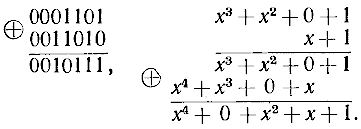
\includegraphics[scale=0.7]{ex_eq}
  \end{figure}
  Отсюда ясно, что при соответствующем выборе образующего многочлена любая разрешенная кодовая комбинация циклического кода может быть получена в результате умножения образующего полинома на некоторый другой полином. Иными словами, любой многочлен циклического кода делится на образующий полином без остатка. Ни один многочлен, соответствующий запрещенной кодовой комбинации, на образующий многочлен без остатка не делится. Это свойство позволяет обнаруживать ошибку. По виду остатка можно определить и вектор ошибки.
  
  Умножение и деление многочленов весьма просто осуществляется на регистрах сдвига с обратными связями, что и явилось причиной широкого применения циклических кодов.
  
  Рассмотрим простейший циклический код, обнаруживающий все одиночные ошибки. Любая принятая по каналу связи кодовая комбинация $h(x)$, возможно содержащая ошибку, может быть представлена в виде суммы по модулю 2 неискаженной комбинации кода $f(x)$ и вектора (кода) ошибки $\xi(x)$:
  \begin{equation}
    \nonumber
    h(x)=f(x)\oplus \xi(x)\text{.}
  \end{equation}
  
  При делении $h(x)$ на образующий полином $g(x)$ остаток, указывающий на наличие ошибки, будет обнаружен только в том случае, если многочлен, соответствующий вектору ошибки, не делится на $g(x)$. Вектор одиночной ошибки будет иметь единицу в искаженном разряде и нули во всех остальных. Ему будет соответствовать многочлен $\xi(x)=x^j$. Последний не должен делиться на $g(x)$. Среди неприводимых полиномов, входящих в разложение $x^n+1$, многочленом наименьше степени, удовлетворяющий указанному условию, является $x+1$.
  
  Для исправления одиночных ошибок или обнаружения двойных существуют циклические коды Хэмминга с $d_\text{мин}=3$, чьи некоторые основные характеристики приведены в таблице ниже.
  \begin{figure}[H]
	  \centering
	  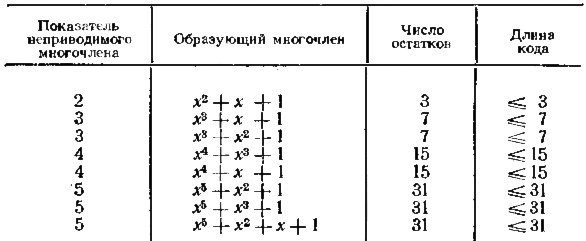
\includegraphics[scale=0.7]{table}
  \end{figure}
  
\subsubsection{Код Боуза-Чоудхури-Хоквингема}
  
  Ранее мы выяснили, что неразложимый многочлен $g(x)$ является порождающим многочленом кода длины $n$, если он делит двучлен $x^n+1$ без остатка, то есть если $(x^n+1)\mod g(x)=0$. Для этого все корни многочлена $g(x)$ должны быть корнями двучлена $x^n+1$. И вообще, корни всех неразложимых многочленов, произведение которых есть двучлен $x^n+1$, также должны  быть  корнями  этого  двучлена.  Общее  количество  его  корней должно быть равно степени этого двучлена. С другой стороны, поскольку любой многочлен $a(x)$, представляющий собой кодовое слово, должен делиться на порождающий многочлен $g(x)$, то все корни порождающего многочлена должны быть корнями многочлена $a(x)$. Но порождающий многочлен неразложим на сомножители, а это должно означать, что  у  порождающего  многочлена  корней  нет.  С  подобным обстоятельством  мы  сталкивались  при  решении,  например,  квадратных уравнений с вещественными коэффициентами, у которых в вещественной области корней не было. В этих случаях приходилось расширять множество вещественных чисел до множества комплексных чисел и находить корни в этом расширенном множестве. В каком же множестве лежат все корни двучлена $x^n+1$? Оказывается, что корнями этого двучлена являются элементы  $\alpha_j=x^j\mod g(x)$.
  
  Коды Боуза-Чоудхури-Хоквингема (коды БЧХ) являются линейными циклическими кодами и представляют собой обобщение циклических кодов. Эти коды позволяют исправлять многократные ошибки и пачки ошибок. БЧХ-коды задаются корнями порождающих многочленов. В качестве порождающих многочленов в этом случае служат приводимые многочлены g(x)=p(x)q(x),  которые  суть  произведения  неприводимых нормированных 
многочленов.
  
  В БЧХ-коде построение образующего многочлена, в основном, зависит от двух параметров: от длины кодового слова $n=m+i$ и от числа исправляемых ошибок $s$.
  
  Особенностью кода является,   то что  для исправления числа ошибок $s\geq 2$ еще недостаточно условия, что между комбинациями кода минимальное кодовое расстояние $d_\text{мин}=2*s+1$. Необходимо также, чтобы длина кода n удовлетворяла условию
  \begin{equation} \label{eq:bch_usl1}
    n = 2h - 1,
  \end{equation}
  где h~-- любое целое число.
  
  При этом $n$ всегда будет нечетным числом и принимать значения: 1, 3, 7, 15, 31, 63, 127\ldots и т.д, т.е не все $i$ могут быть заданы пользователем. 

  Выбранная величина $n$ определяет число контрольных символов $k$:
  \begin{equation} \label{eq:bch_usl2}
    k\leq h*s\leq [\log_2 (n+1)]*s\text{.}
  \end{equation}
    
  При решении задачи выбора допустимого числа информационных символов при заданных корректирующих свойствах удобно пользоваться таблицей, в которой приведены соотношения корректирующих и информационных разрядов для БЧХ кодов.
  
  
\subsection{Ход работы}
  
\subsubsection{Коды Хэмминга}
  
  В MATLAB для кодирования данных с использованием блочных кодов используется функция \textbf{encode}. Кодирование по Хэммингу этой функцией осуществляется с помощью генераторной матрицы $G$. Она получается из второго возвращаемого аргументе функции \textbf{hammen}, вызываемой с параметром, соответствующему числу контрольных бит $k=n-i$ кодируемого сообщения. Затем матрица с информационными битами умножается на $G$ и берется остаток от деления на $2$.
  
  Попробовал закодировать комбинацию $1110$ с помощью \textbf{encode}:
  \begin{lstlisting}
codeA = encode ([1 1 1 0], 7, 4, 'hamming')
  \end{lstlisting}
  Результат~-- столбец $codeA=0101110$. Т.к. используется генераторная матрица, то сомневаться не приходится в том, что первые три бита~-- контрольные, а оставшаяся часть последовательности~-- исходные данные.
  
  Передал в качестве последнего аргумента другую генераторную матрицу вида
\[
  G=
  \begin{pmatrix} 
		1 & 0 & 0 & 0 & 1 & 1 & 0 \\ 
		0 & 1 & 0 & 0 & 1 & 0 & 1 \\ 
		0 & 0 & 1 & 0 & 0 & 1 & 1 \\ 
		0 & 0 & 0 & 1 & 1 & 1 & 1 \\ 
  \end{pmatrix}
\]
  в качестве последнего аргумента функции \textbf{encode}:
  \begin{lstlisting}
G=[1 0 0 0 1 1 0; 0 1 0 0 1 0 1; 0 0 1 0 0 1 1; 0 0 0 1 1 1 1];
codeB = encode ([1 1 1 0], 7, 4, 'linear', G)
  \end{lstlisting}
  Получил кодовую комбинацию $codeB=1110000$, в которой теперь контрольными битами являются три последних.
  
  Декодирование кодов Хэмминга осуществляется функцией \textbf{decode}.\linebreak Она также использует \textbf{hammgen} с числом корректирующих символов $k$ в качестве аргумента для создания как проверочной матрицы $H$, так и генераторной $G$ (первый и второй возвращаемый аргумент соответственно). Далее создается таблица декодирования по матрице $H$ функцией \textbf{syndtable}. Первая строка таблицы декодирования соответствует случаю отсутствия ошибок при приеме. Остальные строки содержат все семь возможных векторов однократных ошибок, исправляемых данным кодом.
  
  Затем определяется синдром путем умножения закодированного сообщения на $H$. Вычисляется позиция однократной ошибки с помощью таблицы декодирования. Производится исправление ошибки и формирование исправленной кодовой комбинации.
  
  Декодировал последовательности $codeA$ и $codeB$ с помощью \textbf{decode}:
  \begin{lstlisting}
dcA = decode(codeA, 7, 4, 'hamming');
dcB = decode(codeB, 7, 4, 'linear', G);
  \end{lstlisting}
  В результате получил $dcA=dcB=1110$, что полностью совпадает с кодовой комбинацией до кодирования.
  
  Попробовал произвести кодирование и декодирование с помощью генераторной и проверочной матриц. Для этого буду также использовать $(7,4)$-код Хэмминга. Выбрал последовательность $0111$.
  \begin{lstlisting}
>> msg = [0 1 1 1];
>> code = rem(msg*G, 2) % кодирование
   code =
        0     1     1     1     0     0     1
>> H = gen2par(G)' % создание проверочной матрицы
   H =
        1     1     0
        1     0     1
        0     1     1
        1     1     1
        1     0     0
        0     1     0
        0     0     1
>> syn = rem(code*H, 2) % синдром
   syn =
     0     0     0
  \end{lstlisting}
  Нулевой синдром сообщает о том, что ошибки не обнаружены. Инвертировал четвертый бит закодированной последовательности $code$ (ошибка смещения), а затем вычислил синдром и позицию искаженного бита:
  \begin{lstlisting}
>> code(4)=~code(4) % инверсия четвертого бита
   code =
         0     1     1     0     0     0     1
>> trt = syndtable(H') % таблица перекодировки
   trt =
        0     0     0     0     0     0     0
        0     0     0     0     0     0     1
        0     0     0     0     0     1     0
        0     0     1     0     0     0     0
        0     0     0     0     1     0     0
        0     1     0     0     0     0     0
        1     0     0     0     0     0     0
        0     0     0     1     0     0     0
>> syn = rem(code*H, 2) % вычисление синдрома
   syn =
        1     1     1
>> err = bi2de(fliplr(syn)) % определение позиции ошибки
   err =
        7
>> err_loc = trt(err + 1, :)
   err_loc =
        0     0     0     1     0     0     0
>> % по err_loc видно, что ошибка в 4м бите
>> ccode = rem(err_loc + code, 2) % исправление
   ccode =
          0     1     1     1     0     0     1
  \end{lstlisting}
  Из кода выше видно, как исправляется единичная ошибка. Теперь можно декодировать комбинацию путем отбрасывания корректирующего кода:
  \begin{lstlisting}
>> i=4; % число инф. бит исходной последовательности
>> rx = ccode(:, 1:i); % тут воспользовались тем, что
                       % положение инф. бит известно
   rx =
        0     1     1     1
>> biterr(msg, rx) % ошибка между исх. и декод. сообщ.
   ans =
        0 
  \end{lstlisting}
  Проверка числа несовпадающих битов дала отрицательный результат~-- во время декодирования успешно обнаружена и исправлена единичная ошибка.
  
  Для оценки корректирующей способности кода определил минимальное кодовое расстояние с помощью встроенной функции \textbf{gfweight}:
  \begin{lstlisting}
>> % gfweight находит d_min разделимого блочного кода.
>> % В качестве пар-тра принимает генераторную матрицу G
>> d_min=gfweight(G)
>> d_min =
        3
  \end{lstlisting}
  $d_\text{мин}=3$, что соответствует теоретическому значению. Из соотношения $d_\text{мин}\geq r+1$ можно найти, что код $(7,4)$ способен обнаружить ошибки кратности $r=2$, а из неравенства $d_\text{мин}\geq 2s+1$~-- исправить ошибки кратности $s=1$. Таким образом, корректирующая способность кода равна одному.

Помимо исследование в среде MATLAB, было произведено кодирование при помощи собственной программы.
Программа на входе получает число, которое необходимо закодировать. На выходе получается закодированное число, и проверка, что число декодируется верно.
Листинг приведен ниже:
\begin{lstlisting}
#include <iostream>
#include <string.h>
#include <math.h>
#include <stdlib.h>
using namespace std;


int takeR(//функция нахождения контрольного бита через таблицу
		const int rNumber,//номер контрольного бита
		string word //кодируемое слово
	){
	int sum=0;//хранит сумму произведений элементов слова и строки таблицы
	bool flag=false;//флаг для задания последовательности элементов в строке
	int step=pow(2,rNumber);//длина шага последовательности элементов
	for(int i=0, j=1; i<(word.length()); i++){
		if(j==step){
				flag=!flag;
				j=1;
			}
			else
				j++;
		if(flag)
			sum+=1*((int)word[i]-48);
	}
	return sum%2;	//возвращает 1, либо 0
}

string encode(string word){//функция кодирования
	if(word.length()==NULL)//отказ, если слово пустое
		return NULL;
	int rNum=1;//хранит количество контрольных бит
	int wordSize=word.length();//длина слова
	for(int i=2; (wordSize+rNum)>=i; i*=2)
		++rNum;
	string newword("0", wordSize+rNum);//временная переменная, хранящая кодированное слово
	for(int i=0, n=rNum, s=wordSize; i<(wordSize+rNum); i++){//цикл, вносящий данные из входного слова в кодированное
		if(i==(pow(2, rNum-n)-1) || i==0){//и вводящее нули в разряды контрольных бит
			newword[i]=48;
			n--;
			continue;
		}
		newword[i]=word[wordSize-s];
		s--;
	}
	for(int i=0, n=rNum; i<(newword.length()); i++){//цикл, находящий контрольные биты
		if(i==(pow(2, rNum-n)-1) || i==0){
			newword[i]=takeR(rNum-n, newword)+48;
			n--;
		}
	}
		return newword;//закодированное слово
}

string decode(string word){//функция декодирования
	if(word.length()==NULL)
		return NULL;
	int rNum=1;
	for(int i=2; (word.length())>=i; i*=2)//поиск количества контрольных бит
	++rNum;
	int err=0;//проверка на ошибку
	for(int i=0; i<rNum; i++){

		err+=takeR(i, word)*pow(2, i);//если err!=0, то в слове ошибка

	}

	if(err && err<word.length()){//если есть ошибка, но ошибка меньше длины слова

		word[err-1]=(!((int)word[err-1]-48)+48);
	}
	string newword="";
	for(int i=0, n=rNum, t=0; i<=rNum+t; i++){//функция, вытаскивающая слово из кодированного вида
		if(i==(pow(2, rNum-n)-1) || i==0){
			n--;
			t++;
			continue;
		}
		newword+=word[i];
	}
	return newword;//декодированное слово

}

int main() {

	string a;//входное слово
	cout<<"Input word: ";
	cin>>a;
	cout<<"\nWord: "<<a<<endl;
	a=encode(a);
	cout<<"Endcode word: "<<a<<endl;
	a=decode(a);
	cout<<"Decode word: "<<a<<endl;
	system("PAUSE");

	return 0;
}
\end{lstlisting}

Пример работы программы

Input word: Input word: 1101
Word: 1101
Endcode word: 1010101
Decode word: 1101

  
\subsubsection{Циклические коды}
  
  Кодирование данных в MATLAB циклическим кодом осуществляется также функцией \textbf{encode}. Для кодирования этой функции нужно передать длину последовательности $n$, число информационных битов $i$, указать метод кодирования ($'cyclic'$ в данном случае). Можно указать порождающий полином.
Однако, было решено закодировать данные при помощи средств языка С. Ниже приведен листинг проекта.
  
  В программном пакете MATLAB есть функция \textbf{encode}, но в связи с принятым решением производить кодирование с помощью языка С, просто опишем каким образом она работает: в том случае, если \textbf{encode} используется для циклического кодирования, сперва определяет, передан ли ей порождающий полином. Если его нет, то вызывается функция \textbf{cyclpoly}, генерирующей порождающий многочлен минимальной длины для заданных $n$ и $i$. Затем с помощью \textbf{cyclgen} формируются порождающая матрица $G$, которая умножается на исходную битовую последовательность со взятием остатка по делению, образуя кодовую последовательность. Это выполняется так же, как в случае с кодом Хэмминга.
  
  Выполнил циклическое кодирование кодом $(7,4)$ с помощью \textbf{encode}:
  \begin{lstlisting}
>> msg=[1 0 1 1]; % пол байта
>> code=encode(msg,7,4,'cyclic')
   code =
        0     0     0     1     0     1     1
  \end{lstlisting}
  Отчетливо видно, что и на этот раз первые три бита являются контрольными, а оставшиеся~-- информационные и соответствуют том, что было передано в $msg$.

Для сравнения выполним циклическое кодирование при помощи следующей программы.
\begin{lstlisting}
#include <stdio.h>
#include <string.h>
#include <stdlib.h>
#include <conio.h>
#include <locale.h>

#define N 15
#define Np 7

// Парсер строки в биты
unsigned long str_to_bits(char* str)
{
    int len = strlen(str);
    unsigned long res = 0;

    for (int i = 0; i < len; i++)
    {
        if (str[i] == '1')
            res++;
        res <<= 1;
    }
    res >>= 1;

    return res;
}
//******************************************
//Паресер битов в строки для вывода
char* bits_to_str(unsigned long num, int k)
{
    char* str = new char[k + 1];
    unsigned long mask = (1 << (k - 1));

    for (int i = 0; i < k; i++)
    {
        if (num & mask)
            str[i]='1';
        else
            str[i]='0';
        mask >>= 1;
    }
    str[k]='\0';

    return str;
}
//******************************************
//Деление полиномов
unsigned long DividePolynoms(unsigned long U, int k, unsigned long P, int p)
{
    int mask = (1 << (k + p - 2));

    P <<= (k - 1);

    for (int i = 0; i < k; i++)
    {
        if (U & mask)
            U ^= P;
        mask >>= 1;
        P >>= 1;
    }

    return U;
}
//******************************************
//Сдвиг
unsigned long Shift(unsigned long U, int k, char direction)
{
    unsigned long mask, shift_bit;

    if (direction == 'l')
    {
        mask = (1 << (k - 1));
        shift_bit = (U & mask) ? 1 : 0;
        mask = ((U & mask) << 1);
        U <<= 1;
        U ^= mask;
    }
    else
    {
        mask = 1;
        shift_bit = ((U & mask) << (k - 1));
        U >>= 1;
    }

    return U + shift_bit;
}
//******************************************
//Поиск пораждающей матрицы
unsigned long* FindGenMatrix(unsigned long P, int k, int p)
{
    unsigned long* G = new unsigned long[k];

    for(int i = 0; i < k; i++)
    {
        G[i] = (1 << (k + p - 2 - i));
        G[i] += DividePolynoms(G[i], k, P, p);
    }

    return G;
}
//******************************************
//Вывод матрицы
void PrintMatrix(unsigned long * matrix, int m, int n)
{
    for(int i = 0; i < m; i++)
    {
        printf("%s\n", bits_to_str(matrix[i], n));
    }
}
//******************************************
//Поиск максимальной длинны кода
int FindCodeDistance(unsigned long * G, int k, int p)
{
    unsigned long  mask;
    int d = k + p - 1, min;

    for(int i = 0; i < k; i++)
    {
        min = 0;
        mask = 1;
        for (int j = 0; j < k + p - 1; j++)
        {
            if (G[i] & mask)
                min++;
            mask <<= 1;
        }
        if (d > min)
            d = min;
    }

    return d;
}
//******************************************
//Поиск веса кода
int FindWeight(unsigned long num, int k)
{
    int w = 0;
    unsigned long mask = 1;

    for (int i = 0; i < k; i++)
    {
        if (num & mask)
            w++;
        mask <<= 1;
    }

    return w;
}
//******************************************
//Главная функция
int main(int argc, char* argv[])
{
	setlocale(LC_ALL,"russian");
    int lenght_of_U = 0;
    int polynom_lenght = 0;
    int d = 0;
    char err[N+1];
    char Ustr[N-Np+1];
    char Pstr[Np+1];
    unsigned long U;
    unsigned long P;
    unsigned long R;
    unsigned long E;
    unsigned long *G;
    unsigned long *H;

	char choise = '0';

			printf("Введите исходное сообщение:\n");
			scanf("%s", Ustr);
			lenght_of_U = strlen(Ustr);
			U = str_to_bits(Ustr);

			printf("Введите пораждающий полином:\n");
			scanf("%s", Pstr);
			polynom_lenght = strlen(Pstr);
			P = str_to_bits(Pstr);

			U <<= (polynom_lenght - 1);
			R = DividePolynoms(U, lenght_of_U, P, polynom_lenght);
			U += R;
			printf("CRC: %s\n", bits_to_str(U, lenght_of_U + polynom_lenght - 1));

			G = FindGenMatrix(P, lenght_of_U, polynom_lenght);
			printf("Пораждающая матрица: \n");
			PrintMatrix(G, lenght_of_U, lenght_of_U + polynom_lenght - 1);

			H = FindCheckMatrix(G, lenght_of_U, polynom_lenght);
			printf("Проверочная матрица: \n");
			PrintMatrix(H, polynom_lenght - 1, lenght_of_U + polynom_lenght - 1);

			d = FindCodeDistance(G, lenght_of_U, polynom_lenght);
			printf("Наименьшее расстояние: %d\n", d);
			printf("Кодирование может обнаружить ошибки уровня %d, правильный уровень ошибок %d\n", d-1, (d-1)/2);

    getch();
    return 0;
}

  \end{lstlisting}

    \begin{lstlisting}
Исходное сообщение: 1101
Пораждающий полином: 111
CRC: 101101
Пораждающая матрица:
100011
010010
001001
000111
Проверочная матрица:
110110
101101
Наименьшее расстояние: 2
  \end{lstlisting}

Как можно заметить, CRC коды различны, однако, при декодировании каждого из кодов в среде матлаб получаются одинаковые исходные сообщения.

  Попробовал получить другую генераторную матрицу, с помощью которой можно осуществить циклическое кодирование $(7,4)$:
  \begin{lstlisting}
>> cyclpoly(7,4,'all')
   ans =
        1     0     1     1
        1     1     0     1
  \end{lstlisting}
  Видно, существует два порождающих полинома. Воспользуюсь вторым: $x^3+x^2+1$.
  \begin{lstlisting}
>> code=encode(msg,7,4,'cyclic',poly)
   code =
        1     0     0     1     0     1     1
  \end{lstlisting}
  
  Декодирование выполняется функцией \textbf{decode}. Ее работа немногим отличается от предыдущего случая. Она использует \textbf{cyclpoly}, если порождающий полином не был передан, для генерации проверочной матрицы $H$ и порождающей $G$ с помощью функции $cyclgen$ (теперь берутся оба возвращаемых аргумента). Далее создается таблица декодирования синдрома. Это делает функция \textbf{syndtable}, использующая матрицу $H$. Дальнейшие действия аналогичны тем, что были в случае кодов Хэмминга: вычисляется синдром, определяется позиция ошибки, коррекция декодируемой последовательности и извлечение информационных бит.
  
  Осуществил декодирование двух блоков, используя \textbf{decode} и сгенерированный ранее порождающий многочлен:
  \begin{lstlisting}
>> rx=decode(code,7,4,'cyclic',poly)
   rx =
        1     0     1     1
>> biterr(msg,rx) % определение числа ошибок
   ans =
        0
  \end{lstlisting}
  Полученные декодированные данные полностью совпадают с тем, что было до кодирования.
  
Теперь проверим CRC программы на С.
\begin{lstlisting}
msg =

     0     1     0     1     0     1

>> code = decode(code, 7, 4, 'cyclic')

code =

     0     1     0     1
  \end{lstlisting}
Как можно заметить, данные совпадают.

   Определение корректирующей способности кода возможно с помощью порождающего многочлена и функции \textbf{gfweight}:
  \begin{lstlisting}
>> wt = gfweight(poly,7) % 7 - длина кодовой комбинации
   wt =
        3
  \end{lstlisting}
  Выяснил, что $d_\textbf{мин}=3$. Выводы, сделанные ранее по кодам Хэмминга, здесь также уместны: корректирующая способность равна одному.
  
\subsubsection{Код Боуза-Чоудхури-Хоквингема}
  
  В MATLAB для кодирования кодом БЧХ можно использовать \textbf{encode}, однако она считается устаревшей и рекомендуют использовать \textbf{bchenc}. Для работы последней функции требуется, чтобы кодируемое сообщение было представлено в поле Галуа.
  \textbf{bchenc} по заданным параметрам $n$ и $i$ генерирует порождающий полином $g(x)$ вызовом функции \textbf{bchgenpoly}. По $g(x)$ строится порождающая матрица с помощью \textbf{cyclgen} (второй возвращаемый аргумент). Затем происходит кодирование путем умножения сообщения на $G$. Брать дополнительно результат умножения по модулю 2 не нужно, т.к. эта операция в полях Галуа делается как раз по модулю 2 (в случае, если размерность поля равна двум, т.е. $GF(2)$).

Однако, нами был написан код на языке Python, который реализует данный алгоритм. Код приведен ниже.
\begin{lstlisting}
from aetypes import end

from bcx_gen import getBCHcodes

a = input('Enter your message (in Decemal):')  # ishodnoe soobchenie
d = input('Enter your Constructive distance (in Decemal):')
g = getBCHcodes(d)  # poragdauchiy polinom

gbin = bin(g)[2:]  # binary string
gbin = gbin[::-1]  # inverting

# make massage
sum = 0
for i in gbin:
    if i == '1':
        sum = sum ^ a
    a = a << 1

print ('\nOut Answer: ' + bin(sum)[2:] + '\n')

# Receive message
error = 0b0000  # make some error
a = sum + error

gdel = g
temp = int(len(bin(sum)[2:])) - int(len(gbin))
gdel = gdel << temp

test = int(len(bin(sum)[2:]))
test = pow(2, test - 1)

print ('In Answer:'),
for i in range(int(len(gbin)), int(len(bin(sum)[2:]) + 1)):
    if a < test:
        print("0"),
    else:
        a = a ^ (gdel >> (i - int(len(gbin))))
        print (1),
    test = test >> 1
print ("\nRest: " + str(a))
\end{lstlisting} 
  
Для проверки работоспособности кода, сравним со значениями, полученными в MATLAB'e.

  Начал кодирования с формирования сообщения в поле Галуа:
  \begin{lstlisting}
>> msg = [1 0 1 1; 0 1 1 1]; % два блока
>> msg = gf(msg) % перевод в поле Галуа
   msg = GF(2) array. 
   Array elements = 
         1      0      1      1
         0      1      1      1
  \end{lstlisting}
  
  Теперь можно выполнить \textbf{bchenc}:  
  \begin{lstlisting}
>> code = bchenc(msg,7,4) % кодирование
   code = GF(2) array. 
   Array elements = 
         1      0      1      1      0      0      0
         0      1      1      1      0      1      0
  \end{lstlisting}
  Получившаяся кодовая комбинация также лежит в поле Галуа. Видно, что первые $i=4$ символов являются информационными, а оставшиеся $k=3$~-- корректирующими. Значения, которые были получены с помощью Matlab и программы, совпали.
  
  Внес в кодовую комбинацию одиночную ошибку, чтобы затем декодировать и убедиться, что БЧХ-код $(7,4)$ позволяет исправить такой тип ошибок:  
  \begin{lstlisting}
>> ncode=code+randerr(2,7) % внесение помех
ncode = GF(2) array. 
Array elements = 
      1      0      1      1      0      0      1
      0      1      0      1      0      1      0
>> rx=bchdec(ncode,7,4) % декодирование
rx = GF(2) array. 
Array elements = 
      1      0      1      1
      0      1      1      1
>> isequal(msg,rx) % проверка на равенство
ans =
     1
  \end{lstlisting}
  Как и ожидалось, код $(7,4)$ справился с обнаружением и исправлением одиночной ошибки.
  
  Попробовал сгенерировать порождающий полином для получения\linebreak других значений помехоустойчивости. Из \eqref{eq:bch_usl1} выяснил, что после длины $n=7$ следует 15. Пусть требуется обеспечить исправление до 2 ошибок, т.е. $s=2$. Из \eqref{eq:bch_usl2} нашел, что число корректирующих бит $k=8$. Тогда информационных бит всего 7. Воспользовался функцией \textbf{bchgenpoly}, которая образует требуемый порождающий полином:  
  \begin{lstlisting}
>> [poly, t]=bchgenpoly(15,7)
   poly = GF(2) array. 
   Array elements = 
         1   1   1   0   1   0   0   0   1
   t =
        2
  \end{lstlisting}
  Получил полином $g(x)=x^8+x^7+x^6+x^4+1$. Также вторым аргументом функция вернула корректирующую способность: она равна двум, как и требовалось.
  
  Далее произвел формирование десяти случайных сообщений длины семь, их кодирование, внесение шума путем сложения с матрицей, генерируемой \textbf{randerr}, декодирование и проверка с исходными сообщениями:
  \begin{lstlisting}
>> msg=gf(randint(10,7,[0 1])); % 10 7-битных чисел
>> code=bchenc(msg,15,7); % кодирование
>> ncode=code+randerr(10,15,2); % внесение по 2 ошибки в строку
>> rx=bchdec(ncode,15,7); % декодирование
>> isequal(rx,msg) % проверка с исходными кодами
   ans =
        1
  \end{lstlisting}
  Таким образом, сформированный полином действительно обеспечивает заявленную корректирующую способность.
  

\subsection{Код Рида-Соломона}

Приведенный ниже код демонстрирует пример работы способа кодирования Рида-Соломона. 
\begin{lstlisting}
#include <iostream>
#include <cmath>

int sum_gf(int a,int b){
    int sum = a + b;
    sum = sum % 7;
    return sum;
}

int pow_gf(int a, int b){

    int pow_table [7][7]={
        {0,0,0,0,0,0,0},
        {1,1,1,1,1,1,1},
        {1,2,4,1,2,4,1},
        {1,3,2,6,4,5,1},
        {1,4,2,1,4,2,1},
        {1,5,4,6,2,3,1},
        {1,6,1,6,1,6,1}
    };
    return pow_table[a][b];
}

int dev_gf(int a,int b){
    a *=b;
    b *=b;
    int dev =a/(b%7);
    return dev%7;
}



int main() {

    int size = 2;
    int input[2] = {3,1};
    int ness_size = 2 *2 + size; // num of errors * 2

    int full_message[ness_size];
    int send_message[ness_size];

    //генерация передаваемого сообщения
    for (int i = 0; i < ness_size; i++) {
        full_message[i]=0;
        send_message[i]=0;
    }
    //закидываем начало сообщения из импута
    for (int i = 0; i < size; i++) {
        full_message[i]=input[i];
    }
    //проверка
    std::cout << "Take this:";
    for (int i = 0; i < ness_size; i++) {
          std::cout << full_message[i] << " " ;
    }std::cout <<" \n";

    //Примитивный элемент
    int Z = 5;

    //Преобразование Фурье
    for (int j = 0; j < ness_size; j++) {
        int temp_sum = full_message[0];
        for (int i = 1; i < ness_size; i++) {
            temp_sum = sum_gf(temp_sum, pow_gf (Z,j)* full_message[i]);// Тут сделать правильное умножение!!!
        }
        send_message[j] = temp_sum;
    }

    //проверка
    std::cout << "Send this:";
    for (int i = 0; i < ness_size; i++) {
          std::cout << send_message[i] << " " ;
    }
    std::cout << "\n" ;

    //Получили сообщение с ошибкой
    // Ошибка= (0,0,0,2,0,6), получим сf(4,1,0,4,5,5).
    int resive_message[6] = {4,1,0,4,5,5} ;



    //Преобразование Фурье
    for (int j = 0; j < ness_size; j++) {
        int temp_sum = resive_message[0];
        std::cout <<temp_sum<<" ";
        for (int i = 1; i < ness_size; i++) {
            std::cout << i*j<<"|";
        }
        send_message[j] = dev_gf(temp_sum,6);
        std::cout<<"\n";
    }
    //проверка
    std::cout << "Send this:";
    for (int i = 0; i < ness_size; i++) {
          std::cout << send_message[i] << " " ;
    }

    return 0;
}
  \end{lstlisting}
Пример работы программы:
\begin{lstlisting}
Take this:3 1 0 0 0 0  
Send this:4 1 0 2 5 6 
4 0|0|0|0|0|
4 1|2|3|4|5|
4 2|4|6|8|10|
4 3|6|9|12|15|
4 4|8|12|16|20|
4 5|10|15|20|25|
Send this:3 3 3 3 3 3 
\end{lstlisting}

в MATLAB'e Кодирование Рида-Соломона осуществляется с помощью rsenc. Можно
воспользоваться функцией encode, однако ее применение не рекоменду-ется. Для работы rsenc требуется, как и в случае с кодированием БЧХ,
чтобы исходное сообщение было представлено в поле Галуа GF ($2^s$), где s – число бит на символ. При этом длина n закодированного сообщения определяется выражением $2^s -1$.
 
  
\subsection{Вывод}

В теории информации выделяют три вида преобразования информации: криптографическое шифрование, помехоустойчивое кодирование и сжатие (или эффективное кодирование). Общим для всех трех видов преобразования является то, что информация каким-либо образом меняет форму представления, но не смысл. Отличия разных видов кодирования связаны с целью проводимых преобразований.

Так, целью криптографического преобразования является, как известно, защита от несанкционированного доступа, аутентификация и защита от преднамеренных изменений. Помехоустойчивое кодирование выполняется с целью защиты информации от случайных помех при передаче и хранении. Для этого при записи и передаче в полезные данные добавляют специальным образом структурированную избыточную информацию, а при чтении (приёме) её используют для того, чтобы обнаружить или исправить ошибки. Естественно, что число ошибок, которое можно исправить, ограничено и зависит от конкретного применяемого кода.

Эффективное кодирование (или сжатие информации) представляет собой процесс преобразования исходного сообщения из одной кодовой системы в другую, в результате которого уменьшается размер сообщения. Алгоритмы сжатия информации делятся на две группы: алгоритмы сжатия без потерь (обратимого сжатия) и алгоритмы сжатия с потерями (необратимого сжатия). За счет эффективного кодирования уменьшается избыточность сообщений, что позволяет производить более надежное криптографическое шифрование информации.

Таким образом, криптографическое шифрование, помехоустойчивое кодирование и сжатие отчасти дополняют друг друга и их комплексное использование помогает эффективно использовать каналы связи для надежной защиты передаваемой информации.

Данная работа была создана путем сложения усилий трёх студентов. Все коды программ написаны вручную. Отсюде следует, что максимаьлное число повторений одинаковых очтетов == 3. Все остальные отчеты - клоны. 

Авторы: Никитин А.Е., Чупин Н.С., Поляков К.О.
  
\end{document}